\chapter[Melodic detail in production]{Melodic detail in production}\label{sec2}
An essential ingredient of any phonological account of intonation is the definition of a finite set of units which serve as primitives. The combination of these units into higher level structures is then governed by a grammar which specifies paradigmatic and syntagmatic relationships among those primitives, and yields an abstract representation of well-formed structures. This representation, in turn, serves as the input for the stage of phonetic implementation, ultimately generating an output which is comparable with features extracted from the signal. In the model which served as the basis for the development of the Autosegmental-Metrical (AM) framework \cite[10]{pierrehumbert1980phonology}, a finite state grammar generates tunes which are composed by sequences of only two tones (the primitives, namely High and Low). Further rules specify the phonetic implementation of the abstract tune, turning a sequence of discrete labels into a continuous representation which can be analysed in conjunction with fundamental frequency tracks extracted from the signal.

The individuation of a basic inventory of primitives, the specification of the rules governing their selection and combination, and the description of the interface between the phonological and phonetic representation are issues of central interest to every phonological model of intonation, even if the three points can be more or less stressed out in different frameworks. However, these issues are so closely intertwined that drawing a clear line between them is nothing more than a simplifying strategy. Very often, the choices made on a given level end up shaping the account provided for another level. To exemplify, consider Janet Pierrehumbert's early model of English intonation \cite[29]{pierrehumbert1980phonology}, in which the inventory of primitives is restricted to only two tones, as we said above. Given this highly limited set of primitives, we can expect a high degree of complexity in the grammar providing the rules for their combinations. And indeed we find that the two tones can instantiate different structural positions (i.e. pitch accents, phrase accents, boundary tones) within the tune, and that in some cases one given position can be filled up by a combination of tones (as in the case of bitonal pitch accents). On the other hand, we can expect richer inventories to be matched by simpler grammars. This is the case of Pierre Delattre's account of French intonation \citep{delattre1966dix}, in which the primitives are not two tones but ten tonal movements, quite richly specified, namely with regard to the height of their starting and ending point, and to the shape of the contour between them. In this case, the intonational grammar is essentially reduced to a discussion of the paradigmatic aspects (quite linearly linked with syntactic structure and pragmatic meaning) and of some simple syntagmatic restrictions (as in the case of contextually determined allotony).

Thus, trading relations between richness of inventory and complexity of grammar represent a useful lead when describing and contrasting different phonological models of intonation. It is interesting to note that a very similar conceptual device has been proposed when contrasting abstractionist and exemplar models of speech perception. This opposition can be framed in terms of trading relations between richness of representations and complexity of mapping procedures \citep{johnson1997complex}. Under this light, traditional accounts of speech processing would rely on the assumption that listeners derive a ``canonical linguistic representation'' (thus, a simple representation) through a normalization process (a complex mapping) of the incoming speech signal. The collection of abstract representations of this sort would build up the mental lexicon, in which only linguistically contrastive information is stored. In the alternative view, listeners would store many and highly detailed traces for (or as) individual entries in the mental lexicon (complex representations), and access to category labels and meaning would be mediated by a simple similarity function (simple mapping). The adoption of such an exemplar approach allowed Keith Johnson to propose an account of vowel perception \citep{johnson1997speech} in which speaker normalization is no longer necessary: variability in the signal is not regarded as noise preventing the access to an abstract representation, but is rather seen as a resource for robust categorization.

There is a striking parallel between trading relations in complexity among inventory and grammar (in phonological models of intonation) and among representations and mapping (in models of speech perception). This seemed an ideal starting point for a closer examination of the role of prosodic detail in the AM framework.

\section{Introduction}\label{sec21}
In the frame of the AM theory of intonation, phonetic (continuous) \textit{f0} data are translated into a phonological (discretized) tune, composed by the combination of only two tones, labelled as High (H) or Low (L). Intonation contours consist of a string of tonal events linked to the prosodic structure of the sentence: tones can be associated either with prominent syllables (as in the case of pitch accents) or with the edges of various prosodic domains (as in the case of phrase accents and boundary tones). Some tonal events, mainly pitch accents, can phonetically appear as a rise (or a fall) in the \textit{f0} curve. In these cases, they are analysed as the succession of two tones (L H for rises, H L for falls)\footnote{See \citet{dimperio1999tonal} for Neapolitan Italian. Similar treatments have been proposed also for Spanish \citep{hualde2002intonation,face2001focus} and English \citep{ladd2003sagging}.}. In AM, the \textit{f0} path between the two tones which compose a rising pitch accent is not regarded as phonologically relevant. Speech synthesis systems based on this framework \citep{pierrehumbert1981synthesizing,anderson1984synthesis,black1996generating} use a simple monotonic interpolation between the two tones. Nonetheless, data from Neapolitan Italian \citep{dimperio2008phonetics} show that, in different pragmatic contexts, the intonation contour of the same segmental string also differs systematically in terms of the \textit{f0} path between the two tones. The curve seems to follow a concave or convex\footnote{Note that, following the common geometrical terminology, the attributes of concave and convex refer to the half-plane \textit{above} the curve, whereas some of the linguistic literature on the topic uses the opposite viewpoint (see \citealt{grice2000place,dombrowski2005acoustic} for recent examples).} path, depending on the pragmatic context in which the sentences are uttered.

\begin{figure}
\centering
\resizebox{\linewidth}{!}{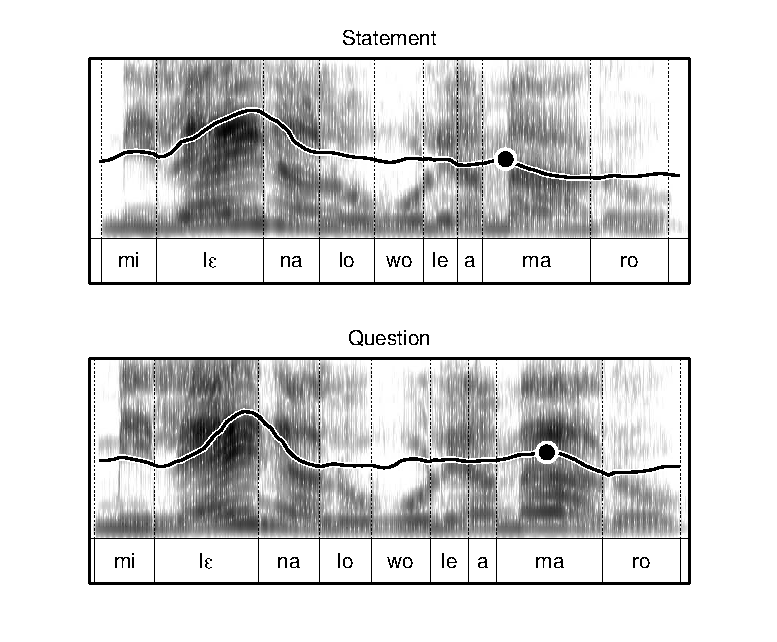
\includegraphics{images/201.pdf}}
\caption{Spectrogram, \textit{f0} track and phonetic transcription of syllable segmentation of the sentence \textit{Milena lo vuole amaro} uttered as a statement (top panel) and as a question (bottom panel).}
\label{fig201}\end{figure}

Figure~\ref{fig201} displays the spectrogram and the \textit{f0} contour for the sentence in (\mex{1}) read twice by a female speaker. 

\ea
\gll Milena lo vuole amaro\\
Milena it wants sour\\
\glt ‘Milena prefers black coffee’
\z

In the first case (top panel), the sentence is uttered as a statement, while in the second it is uttered as a question (bottom panel). From a phonetic point of view, the most striking difference between the two \textit{f0} contours is visible in the movement associated to the last stressed syllable of the sentence (\textipa{/\textvbaraccent{}ma/} in \textit{amaro}). In the top panel we find a gradual fall, while in the bottom one we find a slight rise followed by a quite rapid fall. In other words, the local \textit{f0} peak (marked with the black circles in the figure) occurs slightly before the vowel onset in the statement, but is found later (vowel-internal) in the question, where it is also visibly higher. Following the usual terminology, the H belonging to the post-nuclear pitch accent is aligned (in time) and scaled (in frequency) differently in the two contexts.

Tone alignment and scaling are the indices usually employed in AM to define the phonetic properties of different phonological units (e.g., of the different tones composing a pitch accent). But if we concentrate on the intonation contour of the first word in the sentence (\textit{Milena}), we notice that the rising movement associated with the stressed syllable has a different shape in the two contexts, namely a concave rise in the statement condition and a convex one in the question (\textipa{/\textvbaraccent{}lE/} in \textit{Milena}). This difference, though, does not seem to be related either to the alignment or to the scaling of the two tones: both Ls are in the first half of the stressed syllable onset, and around 225 Hz; both Hs are at the end of the stressed syllable nucleus, and around 350 Hz. Thus, differences in shape of the \textit{f0} contour between the two tones composing the rising pitch accent are not accounted for by the phonetic indices of alignment and scaling employed in AM, and this entails \textit{a fortiori} that shape differences do not play any phonological role in this framework.

In terms of the speech perception models evoked above, we could say that the listener is supposed to ignore the phonetic information provided by the shape of the \textit{f0} contour between tones when categorizing the incoming signal into the different pitch accent options. That is, representations of pitch accents do not include the prosodic detail of interpolation path, which has to be stripped away from the signal during the mapping phase. The autosegmental-metrical model of intonation combines simple primitives using a rich grammar and maps the incoming signal to simplified and underspecified representations, thus qualifying as an overtly abstractionist model. But in this specific case, it appears that the phonetic information retained by the model (scaling and alignment of the tones composing the rise) is less powerful in distinguishing two pragmatic contexts than the information which is discarded (shape of the interpolation between the tones). If shape differences are consistently produced by speakers and consistently used by listeners as a cue to phonological forms with different pragmatic meanings, then the model would need some refinement (by enriching the abstract representations for pitch accents) or even a radical revision (by weakening the abstractionist component).

Building on the results presented in a previous small-scale production study \citep{cangemi2009phonetic}, in this chapter we will compare the traditional AM phonetic indices (namely tone scaling and alignment) with an indicator of contour shape as for their efficacy in discriminating between pragmatic contexts. The analysis of production data will be preceded by a phonological description in AM terms of the materials used in the study (Section~\ref{sec212}), and will be followed by a discussion of the possible impact of our findings on the fine-tuning of the model, in which we will also provide an in-depth review of three studies reporting related findings \citep{dombrowski2005acoustic,petrone2008tonal,petrone2014intonation}. We will conclude the chapter with a discussion of the role of prosodic detail in the reconfiguration of the relationships between phonetic substance, phonological form and pragmatic function in intonation.

\subsection{Hypotheses}\label{sec211}
Before proposing to enrich the description of Neapolitan Italian intonation by adding contour shape information in its phonological representations, we must show that shape differences are consistently produced by speakers and exploited by listeners. The analysis of the perceptual role of contour dynamics (where dynamic refers to properties of \textit{f0} movements rather than of \textit{f0} targets) will be postponed to Section~\ref{sec3}; in the present chapter we will focus on speakers' productions. Indeed, differences in shape could arise as a by-product of the variation in proprieties of tones which are already traditionally acknowledged, namely their alignment and their scaling. For this reason, our first concern will be to evaluate whether the traditional indices of scaling and alignment are adequate in cueing two different pragmatic contexts. We can prospect four scenarios:

\begin{description}
   \item[TD:] \textit{both traditional and dynamic indices} consistently mirror pragmatic contrasts. In this case, the dynamic index could be deemed as redundant, and further elaboration would be pointless.
   \item[TX:] \textit{traditional indices} mirror pragmatic contrasts, while the dynamic one does not. In this case, observations stemming from the informal analysis of material such as the utterance pair in Figure~\ref{fig201} would qualify as statistically aberrant. Again, further elaboration would be pointless.
   \item[XD:] \textit{dynamic indices} mirror pragmatic contrasts, while the traditional ones do not. In this case, before proceeding to the enrichment of phonological descriptions, a perceptual validation is in order.
   \item[XX:] \textit{neither traditional nor dynamic indices} mirror pragmatic contrasts. In this case, either the pragmatic contrast is not instantiated in the phonological position under exam (and any further elaboration would be pointless), or a different dynamic index should be tested. A perceptual test could be used to tell apart these two sub-cases.
\end{description}

In what follows, a corpus of read speech will be analysed in order to find which of these hypotheses is supported. Given the unfortunate condition of a very restricted number of experimental observations available, the operationalization of the hypotheses will be fairly straightforward for this experiment. Indices will be deemed as mirroring pragmatic contrasts if the difference between their means across pragmatic conditions is significantly different (see Section~\ref{sec23}).

\subsection{Phonological analysis}\label{sec212}
Though the main concern of this chapter is with the evaluation of phonetic indices to pragmatic contrasts, given the very nature of our investigation a thorough phonological analysis of the materials used in the experiment is in order.
Over the last decade, NI intonation has been fruitfully studied using the AM framework: both broad surveys and in-depth studies are available to the reader (see Section~\ref{sec123}). Since the original framework was tailored on the specificities of American English intonation, its adaptation to NI required a conspicuous effort and was achieved through the introduction of various more or less innovative features. While a detailed account of the history of these innovations clearly falls outside the scope of this paragraph, we will motivate the main non-standard interpretative devices used in the phonological analyses that follow.

\begin{figure}
\centering
\resizebox{\linewidth}{!}{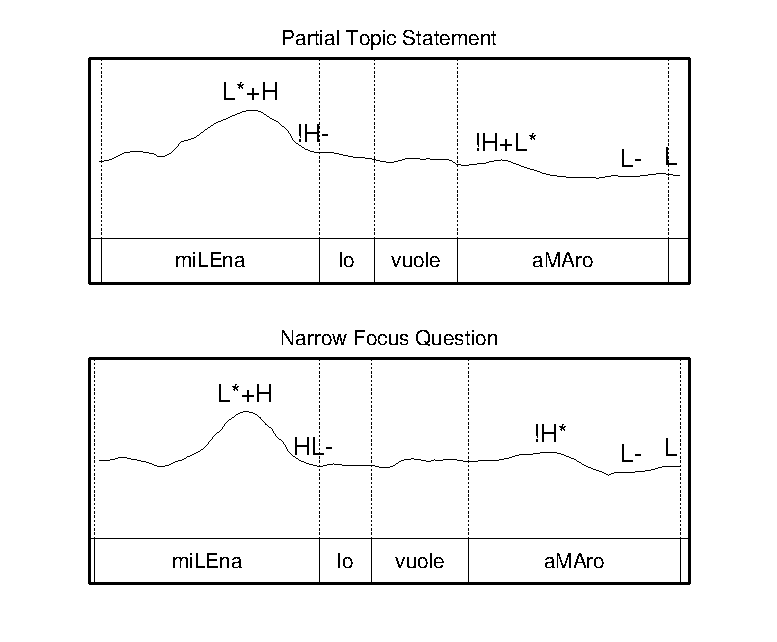
\includegraphics{images/202.pdf}}
\caption{Intonation analysis and word segmentation of the sentence \textit{Milena lo vuole amaro} uttered as a partial topic statement (top panel) and as a subject narrow focus question (bottom panel). Capital letters indicate syllables associated with a pitch accent.}
\label{fig202}\end{figure}

\subsubsection{Pragmatic contexts}\label{sec2121}
Figure~\ref{fig202} shows the \textit{f0} track of the two utterances already displayed in Figure~\ref{fig201}, along with a tonal labelling. In the first case (top panel), the target sentence in (\mex{2}) was uttered as an answer to the question in (\mex{1}). This means that the pragmatic interpretation of the sentence is supposed to be that of a Partial Topic \citep{buring1997meaning}, namely the one in (\mex{3}).

\ea
\gll Come lo bevono il caffè, i tuoi amici?\footnotemark\\
How it drink the coffee, the your friends\\
\footnotetext{The non Neapolitan reader should keep in mind that coffee in Naples is often served already mixed with a sugar-based foam, and that in some cases this is even the ``unmarked'' option. Polite bartenders and hosts, however, are always supposed to ask for a confirmation before serving coffee.}
\glt ‘How do your friends like their coffee?’
\z

\ea
\gll Milena lo vuole amaro\\
Milena it wants sour\\
\glt ‘Milena drinks it black’
\z

\ea
\gll Milena lo vuole amaro, gli altri non saprei\\
Milena it wants sour, the others not know.COND.1SG\\
\glt ‘As for Milena, she drinks it black; as for the others, I wouldn't know’
\z

The new information in the answer (``black coffee'') can be retrieved by analysing the question, which explicitly puts in discussion how the coffee should be served. However, the answer elaborates on the given information as well: among the original set put forth as the topic of the question (``your friends''), the speaker elects a single element (``Milena'') as the subject of the predication. The topic in the answer is thus a subset of the topic in the question: for this reason, in the following we will refer to this context as Partial Topic Statement (henceforth \textit{SPT}). 

The other utterance (Fig.~\ref{fig202}, bottom panel) is labelled as Narrow Focus Question (henceforth \textit{QNF}): in this case, the sentence is imagined to fit in a context where the speaker is serving coffee and remembers that one of his guests (possibly Milena) takes no sugar, and then asks whether she is indeed the one who has to be served black coffee. We will come back to the nature of this pragmatic contrast in the discussion of the link between post-lexical meaning and intonational contrasts (see Section~\ref{sec243}).

\subsubsection{Pitch accents}\label{sec2122}
Two of the stressed syllables in the utterances bear a pitch accent, namely the penultimate in \textit{Milena} and in \textit{amaro}. The first pitch accent in both utterances is nuclear, in the sense that it falls on the rightmost (here, the only) stressed syllable of the focussed constituent \cite[380]{grice2005strategy}. This definition applies in a straightforward way to the QNF context, in which the Subject (\textit{Milena}) is indeed focussed. In the SPT context, however, the Subject is not focussed, but is rather interpretable as a contrastive or partial topic. Since partial topics have been shown to trigger post-accentual compression \citep{dimperio2011phrasing}, they can also be considered as nuclear, and for this reason the pitch accent on \textit{amaro} can be deemed as post-nuclear and transcribed in both cases using a diacritic for range compression (!). This latter pitch accent is different in the two utterances: according to \citet{grice2005strategy}, we use H+L* for the statement and H* for the question; this contrast accounts for the phonetic differences in the scaling and alignment of the high turning point, which were already discussed above (Section~\ref{sec21}). 

As for the first pitch accent, the choice of using the label L*+H for both utterances is consistent with the null hypothesis that shape differences do \textit{not} participate in the specification of pitch accents, are not contrastive and can not justify the use of two different labels. For these reasons, according to \citet{dimperio2008phonetics}, the only paradigmatic choices available in this position would be LH* for the non-contrastive topic rise, L+H* for the focussed statement rise and L*+H for the focussed question rise. Given that the assessment of the phonological status of this rising pitch accent in partial topic statements is one of the main aims of this chapter, we believe that when deciding upon this working hypothesis transcription the safest choice is to rely on the phonetic similarity between pitch accents. For this reason, given the scaling and alignment properties of both tones composing the rise, the nuclear accent in partial topic statements will also be labelled as L*+H at this stage.

\subsubsection{Edge tones and phrasing}\label{sec2123}
Unlike many languages, NI does not mark questions with an high boundary tone, as in the case of many Italian regional varieties \citep{savino2012intonation}. This accounts for the (mainly phonetic) transcription of L\% for both the question and statement; the same holds for the immediately preceding L- phrase accent. 

More importantly, both utterances can be analysed as an intonational phrase composed by two intermediate phrases, namely [(\textit{Milena})(\textit{lo vuole amaro})]. The phrase break after the Subject is expected in the case of the narrow focus question, where the Subject is coextensive with the focus domain. For this same reason, the break would not be expected in broad focus questions \citep{dimperio2005intonational,frota2007phonetics}, nor in non contrastive topic statement, as in the answer to the question in (\mex{1}):

\ea
\gll Milena come lo vuole il caffè?\\
Milena how it wants the coffee\\
\glt ‘How does Milena drink her coffee?’
\z

However, after the Subject in partial topic utterances we find a strong degree of \textit{f0} compression \citep{dimperio2011phrasing}, and in some utterance even a short pause; for these reasons, we assume that there is indeed a phrase accent after the subject in both context, which we label HL- in the case of the narrow focus question, following \citet{dimperio2002italian} and !H- in the case of the partial topic statement, following \citet{dimperio2011phrasing}; see Section~\ref{sec123}.

\section{Method}\label{sec22}
\subsection{Corpus}\label{sec221}
For our study we used a subset of the corpus \textit{Tre Grazie}, first described in \citet{dimperio2008phonetics}. Nine native speakers of NI read 60 experimental stimuli and 38 fillers in a silent room. The stimuli consisted of 5 repetitions of 3 sentences designed without voiceless plosives, which were semantically plausible and syntactically quite similar (\mex{1}--\mex{3}):

\ea
\gll Amelia dorme da nonna\\
Amelia sleeps at grandma\\
\glt ‘Amelia sleeps at grandma's’
\z

\ea
\gll Valeria viene alle nove\\
Valeria arrives at nine\\
\glt ‘Valeria arrives at 9’
\z

\ea
\gll Milena lo vuole amaro\\
Milena it wants sour\\
\glt ‘Milena drinks it black’
\z

Target words were all feminine proper names (hence the corpus' name), agents, subjects, trisyllabic, with penultimate stress, the same syllabic structure for the tonic syllable (.CV.) and the same quality for its nucleus (/\textipa{E}/), while a greater flexibility was allowed for unstressed syllable structure (post-stressed .CCV in \textit{Valeria}, joined by pre-stressed V. in \textit{Amelia}). Sentences were presented together with a contextualization paragraph, which had to be read silently; this made possible the elicitation of every sentence with four different pragmatic meanings. For example, the sentence in (\mex{0}) would be interpreted and uttered by speakers as a QNF with the meaning of (\mex{1}b) if preceded by the context in (\mex{1}a):

\eal
\ex After a family lunch, you’re preparing coffee. You know that one of your cousins is on a diet and stays away from sugar, but you don’t remember which one. You ask your aunt:...
\ex Is it Milena, the one who drinks unsweetened coffee?
\zl

On the other hand, sentences preceded by the context in (\mex{1}a) would be interpreted and uttered as a SPT, with the meaning of (\mex{1}b):

\eal
\ex In the afternoon, among friends, your brother is preparing coffee. He asks you whether your friends would like it sweetened or not. You don’t know everybody’s preferences, but only your girlfriend’s. You answer:...
\ex As for Milena, she drinks it unsweetened; as for the others, I couldn't tell.
\zl

Other contextualization paragraphs prompted a Broad Focus Statement and a Narrow Focus Statement interpretation. In the first case, all the information in the utterance was intended to be new; in the second, the utterance was intended as a statement where the speaker corrects the interlocutor's beliefs about who asked for black coffee (i.e., Narrow Focus is on the Subject).

Given the poor quality of some of the recordings and the focusing on the pitch accents with similar alignment and scaling proprieties for the two tones composing the rise, the experimental material retained for this study consisted of 2 subjects x 3 sentences x 2 pragmatic contexts (QNF and SPT) x 5 repetitions = 60 items total.

\subsection{Measures}\label{sec222}
Target words were manually labelled in syllables using a scripted procedure under \textit{Praat} \citep{boersma2008praat}. The stressed syllable, which always had a CV structure, was also labelled in segments: the labels were \textit{Os} for the beginning of the onset (and of the entire syllable), \textit{Ns} for the beginning of the nucleus (or the end of the onset) and \textit{Ne} for the end of the nucleus (and of the entire syllable)\footnote{See Figure~\ref{fig203}: \textit{Os}, \textit{Ns} and \textit{Ne} on x-axis.}.

\begin{figure}
\centering
\resizebox{\linewidth}{!}{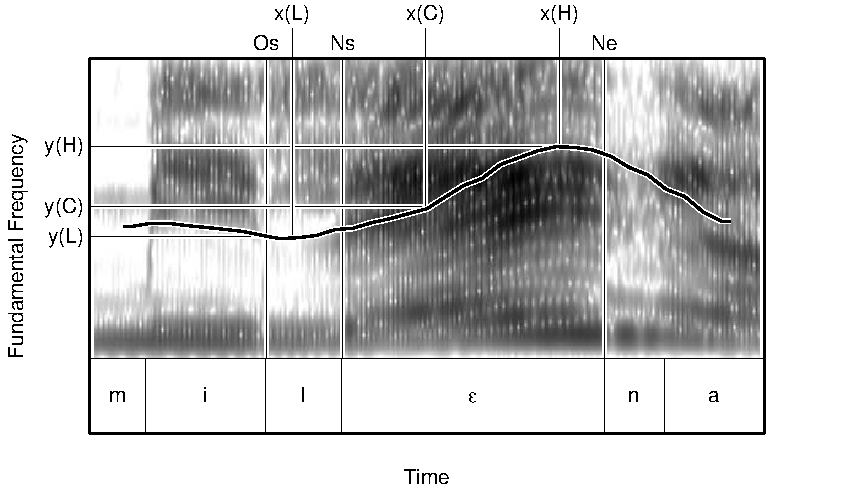
\includegraphics{images/203.pdf}}
\caption{Example of acoustic measures.}
\label{fig203}\end{figure}

The rising \textit{f0} movement in the stressed syllable was characterized by measuring the height (in Hz) and the position in time of its starting and ending points (L and H)\footnote{See Figure~\ref{fig203}: \textit{y(L)} and \textit{y(H)} on y-axis for height (scaling), and \textit{x(L)} and \textit{x(H)} on x-axis for position (alignment).}. Hs were automatically located at \textit{f0} maxima inside the stressed vowels, while the detection of Ls proved more challenging, as could be expected \citep{delgiudice2007comparing,petrone2009tonal}. A widely used automatic procedure is based on the detection of the local minima in the stressed syllable onset, but we found this method too sensitive to microprosodic perturbations at the consonant-vowel boundary. We determined that another strategy for the detection of Ls, the two-lines regression or Least Square Fitting algorithm, used for example in \citet[92-93]{dimperio2000role}, was not suited for our goals either.

\begin{figure}
\centering
\resizebox{\linewidth}{!}{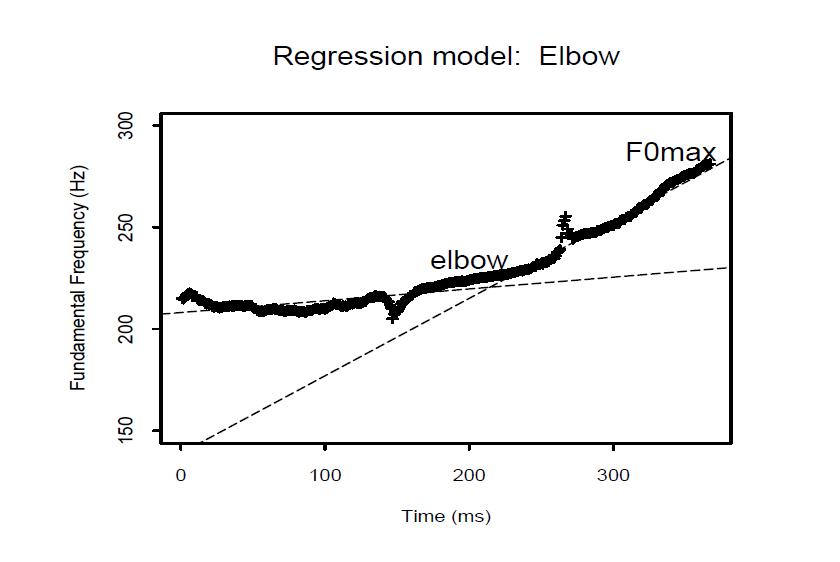
\includegraphics{images/204.png}}
\caption{Two-line fitting (from D'Imperio 2000: 95).}
\label{fig204}\end{figure}

With this technique, the region in which the L must be found (in our case, the \textit{f0} stretch from utterance start to H) is divided into steps. For each point, two straight lines are fitted with a linear regression to the contour on its left and on its right. The time of the L is chosen as the point associated with the pair of lines leading to the smallest modelling error. Since the differences between a concave and a convex rise have consequences on modelling and errors, the algorithm often locates Ls away from the point in which the \textit{f0} curve visibly bends upwards (the \textit{elbow}). Concave shapes tend to be associated to an L on the left of the elbow, and for convex ones the L is detected on its right. This means of course that we would still have an index to express our differences in interpolation, but in this case the information is conveyed in an implicit and indirect way: different shapes are translated into different position of a same tonal target.
We decided to use a method which would ignore the specifically local features of the \textit{f0} contour (such as microprosodic minima) and at the same time avoid the implicit encoding of the global proprieties we were trying to characterize explicitly (as in the case of the two lines regression). Trying to find a compromise between these two constraints, which ultimately means to find a compromise in the size of the analysis window, we decided to locate the elbows at the point of maximal acceleration of the curve. Through the elaboration of an automated procedure in \textit{R} \citep{r2008r}, the L was located by inspecting the \textit{f0} second derivative, looking for sufficiently wide local maxima.

Although the L detection procedure is innovative, height and position of tone targets remain traditional measures. Besides these, we also calculated the height of the mid-point in time between L and H (C)\footnote{See Figure~\ref{fig203}: \textit{y(C)} on y-axis.}. This allowed us to calculate an index (based on \citealt{dombrowski2005acoustic}) which could express the type of interpolation between the two targets in a simple and explicit way; see Section~\ref{sec223}.

In conclusion, for every experimental item we measured the coordinates of L, C and H in the (time, \textit{f0}) plane.

\subsection{Indices}\label{sec223}
We used these coordinates to calculate various indices (see Table~\ref{tab21}), which had to be compared as for their reliability in discriminating our two pragmatic contexts. In addition to the traditional indexes of scaling (height of L and H) and alignment (distance of L and H from both start and end of, respectively, stressed syllable onset and nucleus), we calculated a Curve Index (\textit{Ci}), expressed as the ratio of the difference between the heights of the intermediate and the starting points, and the difference between the heights of the end and starting points of the rise:

\begin{description}
   \item[] \(Ci=\frac{y(C)-y(L)}{y(H)-y(L)}\)
\end{description}

This index is reminiscent of the Range Proportion (\textit{Rp}), used by \citet{dombrowski2005acoustic} to characterize phonetic variation of phrase-final rises in German task-oriented dialogues (see Figure~\ref{fig205} and Section~\ref{sec241}). 

\begin{figure}
\centering
\resizebox{0.66\linewidth}{!}{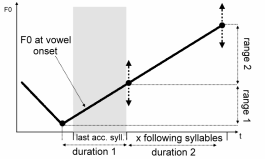
\includegraphics{images/205.png}}
\caption{Range proportion (from Dombrowski and Niebuhr 2005, Fig. 3).}
\label{fig205}\end{figure}

Shape differences in these rises are calculated by dividing the extent of the rise within the stressed syllable by the extent of the rise up to the prosodic phrase boundary. In terms of the labels used in Figure~\ref{fig205}, this means:

\begin{description}
   \item[] \(Rp=\frac{range1}{range1+range2}\)
\end{description}

The main difference between range proportion and curve index resides in the fact that the pivot used for the calculation of the curve index is constantly located at the midpoint in time between the Low and the High tone (Figure~\ref{fig203}), while for the calculation of the range proportion the pivot can move to the left or to the right of the midpoint, according to the position of the stressed syllable right boundary (Figure~\ref{fig205}). Given the nature of their semi-spontaneous corpus, in which the lexical material associated with the phrase-final rises is not controlled neither in quality (syllable structure) nor in quantity (of poststressed syllables), the choice of a moving pivot in Dombrowski and Niebuhr's study is justified. However, since in our read corpus the target words are strictly controlled, we considered that a tighter definition of pivot location could be easily enforced.

\begin{table}[h]
\centering
\resizebox{\linewidth}{!} {
\begin{tabular}{c c c}
Index & Description & Formula \\
\hline
sL & L scaling & y(L) \\
aLs	& L alignment to start of stressed vowel onset & x(L) – Os \\
aLe	& L alignment to end of stressed vowel onset & Ns – x(L) \\
sH	& H scaling	& y(H) \\
aHs	& H alignment to start of stressed vowel nucleus & x(H) – Ns \\
aHe	& H alignment to end of stressed vowel nucleus & Ne – x(H) \\
sC	& C (intermediate point in time between L and H) scaling & y(C) \\
Ci	& Curve index & \(\frac{y(C)-y(L)}{y(H)-y(L)}\) \\
\end{tabular}
}
\caption{Indices}
\label{tab21}\end{table}

\section{Results}\label{sec23}
In this section we plot the distributions of the eight phonetic indices in the two pragmatic contexts for the two speakers. In Figures~\ref{fig206}--\ref{fig208}, columns report data for the two speakers (WP, female, and MB, male) and rows for the indices. The labels used for the indices (on the y-axis) correspond to those used in Table~\ref{tab21}. Each individual plot shows the distribution of an individual index for an individual speaker, separating the two pragmatic contexts (QNF, narrow focus question, and SPT, partial topic statement).

Given the limited amount of data, for the calculation of statistical significance we restrain to two-sample Welch-Satterthwaite t-test. In the absence of inferable biases, the tests were two-tailed. Since data on \textit{f0} height cannot be pooled across our speakers (a male and a female), for uniformity's sake we will split results for alignment as well. Results were pooled across the three sentences and the five repetition of each sentence. Each boxplot thus shows 15 observations.

\subsection{Alignment}\label{sec231}
Figure~\ref{fig206} shows data on alignment of the High tone target relative to the vowel in the stressed syllable (e.g. \textipa{[E]} in the case of \textit{Milena}) and of the Low tone relative to its consonant (e.g. \textipa{[l]} in the same case). Since a preliminary exploration of the data showed that the two tonal targets co-occur with the relative segments, latencies were calculated either by subtracting the startpoint of the Segment (\textit{Ss}) to the timepoint of the Tone (\textit{Tt}) or by subtracting the timepoint of the Tone to the endpoint of the Segment (\textit{Se}): $ aTs = Tt - Ss $ and $ aTe = Se - Tt $. 

\begin{figure}
\centering
\resizebox{\linewidth}{!}{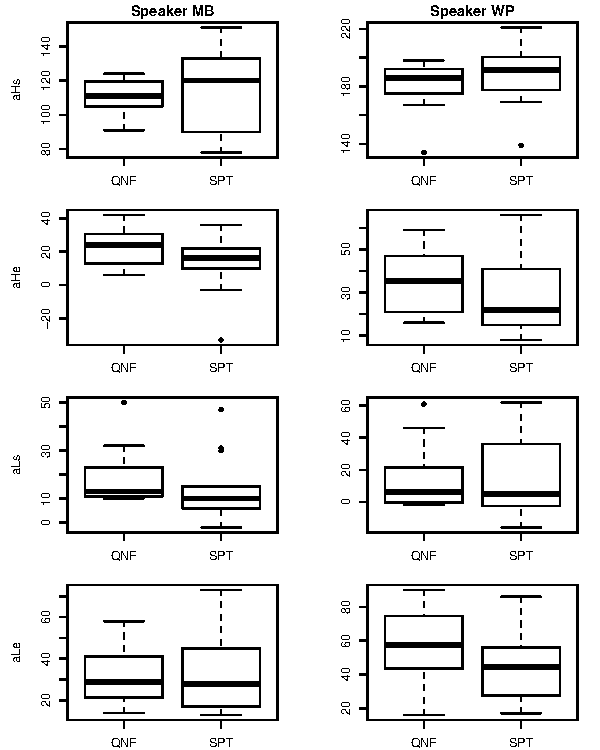
\includegraphics{images/206.pdf}}
\caption{Latencies (ms) from H to vowel onset (first row) and offset (second row), and from L to consonant onset (third row) and offset (fourth row) in stressed syllable.}
\label{fig206}\end{figure}

For both High and Low tones the alignment measures, either to the beginning or from the end of the relevant segment, failed to reliably differentiate between the two pragmatic contexts. As for Hs, the smallest p was above 0.1 (\textit{aHe} for speaker MB), while for Ls it was above 0.15 (\textit{aLe} for speaker WP). Data dispersion around the median appeared to be slightly more compact for questions in both speakers, but the effect was not statistically significant. Hence, tonal alignment does appear to differentiate between partial topic statements and narrow focus questions in NI.

\subsection{Scaling}\label{sec232}
As for tone scaling (Figure~\ref{fig207}), on the other hand, only one plot shows non significant results, namely \textit{Hs} for speaker WP (p$>$0.3). The three other comparisons show a significant difference between the two pragmatic contexts (p$<$0.01). However, in one case (\textit{Ls} for speaker MB) the difference was significant but very small: the mean L height is 92 Hz in questions and 97 Hz in statements. Moreover, this 5 Hz difference always fell inside a consonant, and usually very near to a segmental boundary, as the positive latencies for alignment in Figure~\ref{fig206} (two last left panels) show, thus allowing us to infer that its perceptual role is negligible \citep{house1990tonal}. 

\begin{figure}
\centering
\resizebox{\linewidth}{!}{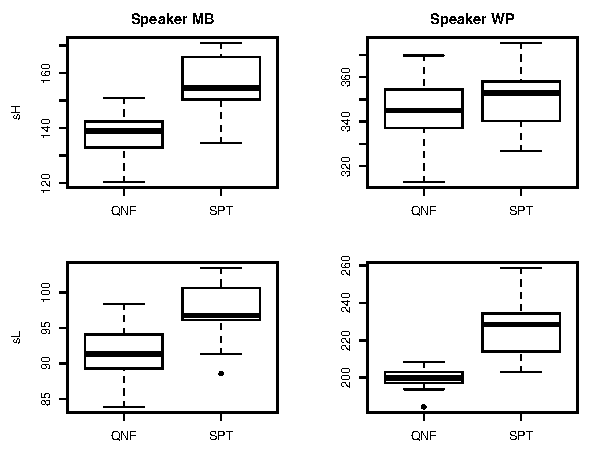
\includegraphics{images/207.pdf}}
\caption{Height (Hz) of High (first row) and Low (second row) tonal target.}
\label{fig207}\end{figure}

As for the two other statistically significant and perceptually relevant comparisons, statements show a higher H tone for speaker MB and a higher L tone for speaker WP. That is, tone scaling information is useful in indicating that both speakers use different \textit{f0} movements in the two pragmatic conditions, but does not yield a unified picture of how these \textit{f0} movements should be characterized. 

\subsection{Shape}\label{sec233}
The indices focusing on contour dynamics show a different picture (Figure~\ref{fig208}). All comparisons were statistically highly significant (highest p is 0.033). Data on scaling, which is perceptually more easily interpretable, show that mean differences between midpoint height (\textit{sC}) in questions and statement was above 40 Hz for speaker WP (female) and above 15 Hz for speaker MB (male). This latter difference can be considered as quite relevant, since speaker MB uses a very narrow pitch span: mean L to H excursion for this speaker is around 40 Hz (compare with a mean excursion of 135 Hz for speaker WP). In relative terms, the differences in C scaling among questions and statements was actually more salient in speaker MB.

\begin{figure}
\centering
\resizebox{\linewidth}{!}{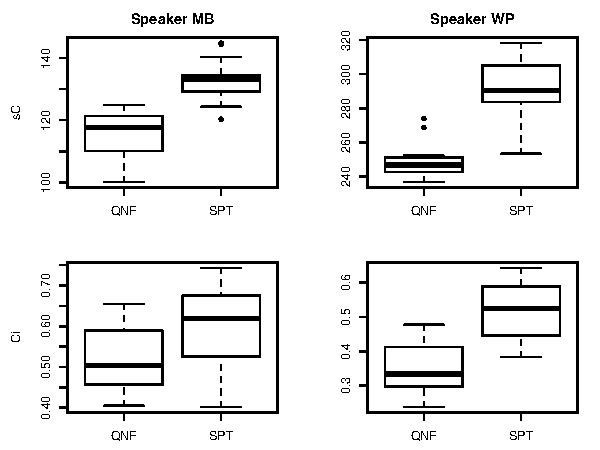
\includegraphics{images/208.pdf}}
\caption{Height (Hz) of midpoint between L and H (first row) and curve index (second row).}
\label{fig208}\end{figure}

Differences in the curve index (\textit{Ci}) might be less straightforward to interpret in perceptual terms than differences in C scaling, but they have at least two advantages. First of all, being a ratio of differences, they do not need any further transformation in order to yield comparable data for speakers with very different pitch spans and ranges. Moreover, differences in curve index can be quite easily interpreted in geometrical terms: a value of 0.5 would indicate a linear interpolation, while values above or below 0.5 would indicate concave and convex rises, respectively. 
In our data, curve index differences are significant for both speakers. The \textit{f0} rise between the L and the H composing the nuclear pitch accent is less concave in QNF contexts (mean \textit{Ci}: 0.52 for MB, 0.35 for WP) and less convex in SPT contexts (mean \textit{Ci}: 0.60 for MB, 0.52 for WP). Thus, even with some individual differences in level and span of curve index variation, we can conclude that speakers tend to show a convex interpolation in questions and to a concave interpolation in statements.

\subsection{Summary of results}\label{sec234}
Among the four scenarios prospected in Section~\ref{sec211} our results support the third, namely that dynamic indices mirror the pragmatic contrast between narrow focus questions and partial topic statements, while the traditional indices of tone scaling and alignment do not.

No significant alignment differences could be found in our corpus, neither for High nor for Low tones, independent of the boundary (left or right) of the relevant segment in the stressed syllable (consonant for Ls, vowel for Hs). Tone scaling appears to be different in the two contexts, but differences are not consistent across speakers: partial topic statements are characterized by higher H tones for speaker MB and higher L tones for speaker WP. Thus, scaling does not qualify as a viable index to our pragmatic contrast. Dynamic indexes, on the other hand, proved robust: both speakers showed a statistically significant tendency to a concave interpolation in statements and to a convex interpolation in questions. 

\section{Discussion}\label{sec24}
In our study, dynamic indices appear to be more consistent than scaling and alignment in mirroring the pragmatic contrast between partial topic statements and narrow focus questions. This finding underlines a potential loss of useful phonetic information in the abstraction procedure that maps  signal onto discrete phonological categories in the AM framework. In this paragraph we will develop this line of thought, by discussing in some detail three other studies as they report previously unaccounted prosodic detail (Section~\ref{sec241}) and prospect different avenues to the enrichment of phonological representations for intonation Section~\ref{sec242}.

\subsection{Contour shape in other contrasts}\label{sec241}
In order to decide whether shape information is a necessary enrichment to phonological representations of intonation, we must evaluate the scope of contrasts which can be expressed exclusively (or more robustly) by dynamic information\footnote{This is not to say that the role of dynamic phonetic detail in \textit{f0} contours has to be reduced to phonological contrastiveness in itself. Recent studies are exploring the interspeaker variability in signalling phonological contrasts, showing that speakers might use different strategies which rely more or less strongly on dynamic cues; see \citet{niebuhr2011shapers}.}. In this experiment we focussed on only one pragmatic contrast, namely the one between narrow focus question and partial topic statement, but recent work on both Italian \citep{dimperio2000role,petrone2008tonal} and German \citep{dombrowski2005acoustic,petrone2014intonation} shows that contour shape could be relevant for other contrasts as well. Interestingly, these studies focus on acoustic and functional differences in structural positions other than the nuclear pitch accents we analysed in this chapter.

\subsubsection{Turn management and utterance final rises in German}\label{sec2411}
In their exploration of the dialogue section of the Kiel Corpus of Read and Spontaneous Speech (\citealt{ipds1994kcrs} and following), for example, \citeauthor{dombrowski2005acoustic} focus on phrase-final rises. They show that a given phonological entity, analysed as an \textit{early valley} in terms of the Kiel Intonation Model (henceforth \textit{KIM}; see \citealt{kohler1991model}), displays a consistent phonetic variation which is best analysed in terms of dynamic proprieties (viz. convexity or concavity of the rise), and that those phonetic variants correlate with two opposite conversational functions (viz. activation or restriction of the interlocutor). Their corpus consisted in task-oriented dialogues in which out of sight participants had to collaborate in scheduling meetings and events; the speakers had access to different sets of partial informations and, crucially, they had to press (and hold) a button near to their individual microphones in order to activate their interlocutor's headphones. This permitted to avoid overlaps, since only one participant at a time was allowed to talk, but more importantly it served as an objectivation of speakers' intentions of turn-yielding (activation) or turn-holding (restriction of the interlocutor). Figure~\ref{fig209} shows an example of a convex rise in a turn-yielding condition (left panel) and a concave rise in a turn-holding condition (right panel)\footnote{Note that in the original paper, contrary to the common geometrical interpretation used in this book, the attributes of concavity and convexity are assigned to the half-plane \textit{below} the curve.}. 

\begin{figure}
\centering
\resizebox{\linewidth}{!}{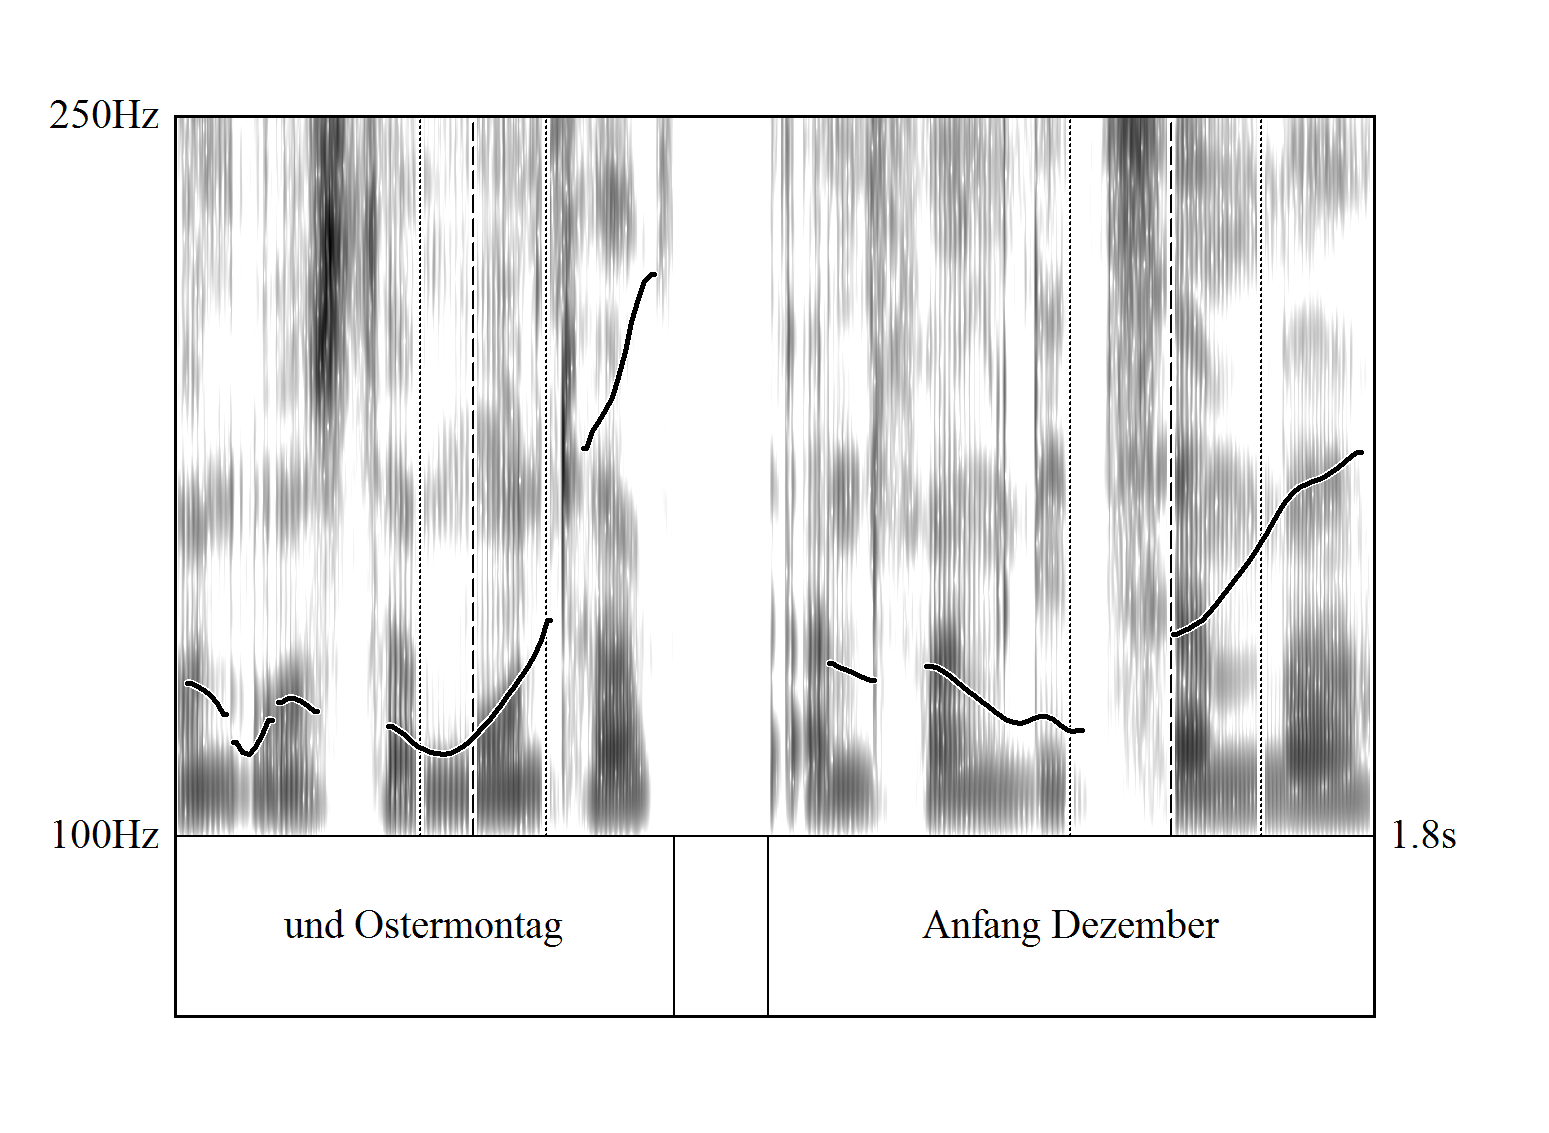
\includegraphics{images/209.png}}
\caption{Activating (left) and restricting (right) final rises (from Dombrowski and Niebuhr 2005, Fig. 1). Grey boxes highlight the accented syllables, vertical lines indicate the accented-vowel onsets.}
\label{fig209}\end{figure}

As we already pointed out (see Section~\ref{sec223}), their phonetic analyses of contour shapes must have been made quite difficult by the lack of control of the number of poststressed syllables and of the syllable structure and, as Figure~\ref{fig209} shows, of voicing throughout the syllable. Figure~\ref{fig209} also shows that, in contrast with our results on Neapolitan Italian nuclear rises, the functional contrast could also be mirrored by alignment and scaling of both rise start- and endpoint, at least for this particular pair of utterances. However, a discriminant analysis showed that the highest correct classification results are achieved when the shape of the rise is the most important predictor.

\subsubsection{Modality and prenuclear fall in Italian and German}\label{sec2412}
Contour shape thus appears to be relevant in \textit{nuclear rises}, both utterance internal (as we have seen in this chapter) and utterance final (as we have seen in the previous section), signalling different pragmatic or conversational contrasts, and in more than one language. In this section we review two studies focusing on the role of contour shape in \textit{prenuclear falls}, respectively in Neapolitan Italian and in Northern Standard German.

Differences in the shape of postnuclear \textit{f0} fall for Neapolitan Italian read speech are connected with sentence modality contrasts in \citet{petrone2008tonal}. Figure~\ref{fig210} shows two utterances (as a statement, top panel and as a question, bottom panel) of the sentence in (\mex{1}), both with narrow focus on the object. 

\ea
\gll La mamma vuole vedere la Bina\\
The mother wants see the Bina\\
\glt ‘Mom wants to meet Bina’
\z

The nuclear accent thus falls on the last stressed syllable (\textipa{\textvbaraccent{}bi.na}), and is labelled as L+H* for the statement and as L*+H for the rise. The prenuclear accent, on the first stressed syllable (\textipa{\textvbaraccent{}mam.ma}), is labelled in both cases as (L)H*, following \citet{gilifivela2003tonal,gilifivela2006coding}. Its rising portion seems to have the same acoustic properties in both contexts; the fall, on the other hand, clearly follows different paths.

\begin{figure}
\centering
\resizebox{\linewidth}{!}{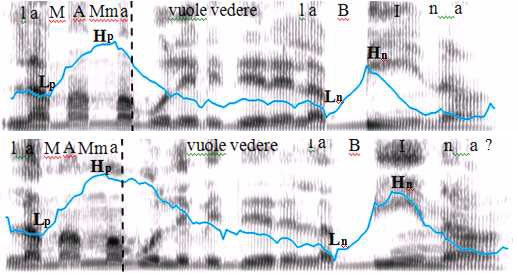
\includegraphics{images/210.png}}
\caption{\textit{f0} contours for (object) narrow focus statement (upper panel) and question (lower panel) utterances of a same sentence (from Petrone and D'Imperio 2008, Fig. 1). Capital letters indicate the stressed syllables; tone targets for prenuclear and nuclear pitch accents are labelled with a subscript \textit{p} and \textit{n}, respectively.}
\label{fig210}\end{figure}

The first half of the tonal stretch between H$_{p}$ and L$_{n}$ can be characterized as convex in the statement and concave in the question. Statistical analyses based on different kinds of regression confirmed the significance of these differences. However, it should be noted that, as in the case of the German activating and restricting contours, alignment and scaling of the tones at both ends of the relevant \textit{f0} stretch are also significantly different in the two contexts: for one of the two speakers, for example, the endpoint of the prenuclear rise (H$_{p}$) is aligned significantly later in questions. 

Very similar results are presented as the starting point of a perception study on Northern Standard German \cite{petrone2014intonation}, which will be examined at length in Section~\ref{sec3}. As in Neapolitan Italian, statements and questions with declarative syntax appear to be characterized by different shapes in the prenuclear fall (respectively, convex and concave). And as in the previous studies, these differences seem to qualify as a reinforcing cue, given that different properties for scaling and alignment are attested as well. Figure~\ref{fig211} shows three utterances of the sentence in (\mex{1}), as a statement (a) and as a question (b-c). 

\ea
\gll Katherina sucht 'ne Wohnung\\
Katherina searches a flat\\
\glt ‘Katherina is looking for a flat’
\z

Apart from utterance (b), which shows a H-H\% sequence at the end of the intonational phrase, the working hypothesis phonological transcription for all utterances is H* L*+H L-L\%, following \citet{grice2002deutsche}. The fall of the prenuclear accent, located on the last syllable of the first word (\textipa{[na]} in \textit{Katherina}), clearly has a different shape in the two contexts (statement vs questions), even if in questions it also starts from a later aligned and lower scaled High tone.

\begin{figure}
\centering
\resizebox{\linewidth}{!}{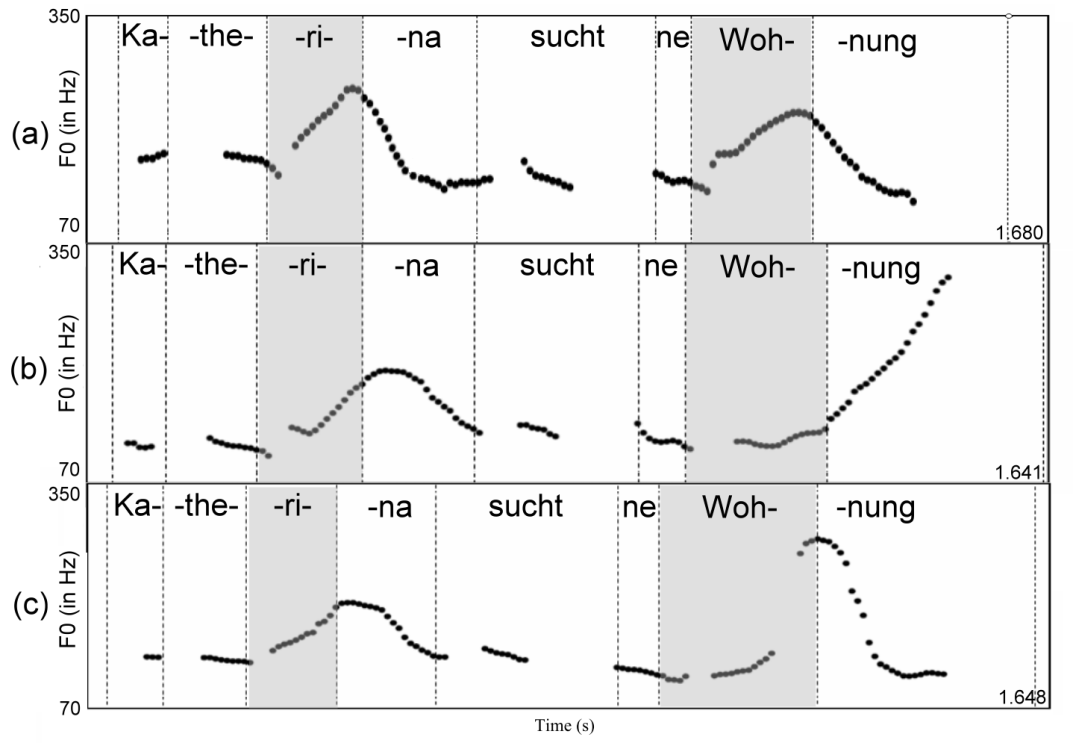
\includegraphics{images/211.png}}
\caption{\textit{f0} contours for statement (a) and question (b-c) utterances of a same sentence with declarative syntax (from Petrone and Niebuhr, forthcoming, Fig. 2). Grey boxes highlight accented syllables.}
\label{fig211}\end{figure}

Thus, shape differences are attested both in other languages and in other structural positions. Moreover, they can be either the sole viable phonetic index to a given contrast, as in our data, or they can act in combination with other cues such as alignment and scaling, as in the studies reviewed in this section. In the next section, we will discuss how these phonetic facts can be accounted for in phonological modelling.

\subsection{Enriching inventories or grammars?}\label{sec242}
Shape differences in the \textit{f0} contour have been shown to match with various pragmatic and conversational contrasts. Now, phonetic differences matching with different functions can be organized in phonological contrasts. And if, as we said in the opening pages of this chapter, phonological accounts of intonation must deal with the intricate relations between grammar and inventories, it becomes clear that no refinement proposal can escape this issue. For example, if we believe shape differences to be a necessary enrichment of phonological representations of intonation, we must ask ourselves whether they should be coded by new entries in the inventory or as new instructions in the grammar.

Among the studies reviewed in the preceding section, the innovations proposed in the AM-based account of prenuclear falls and sentence modality in NI \citep{petrone2008tonal} are a clear example of grammar enrichment. They mirror the general preference for \textit{simple inventory and rich grammar} of the model they are framed in, thus somehow presenting themselves as ``ecologically sustainable'' innovations. \citeauthor{petrone2008tonal} suggest that differences in the shape of the prenuclear fall should be accounted for by a different tone specification, namely a Low tone for statements (yielding a convex fall) and a High tone for questions (yielding a concave fall)\footnote{This choice has also the advantage of being compatible with ethologically based accounts of the grammaticalization of the statement-question contrast, according to which questions are cross-linguistically more likely to be marked by a high tone somewhere in the utterance \citep{ohala1983cross,gussenhoven2004phonology}. We will come back to this issue in the next chapters (see especially Section~\ref{sec451}).}. In an inventory enrichment perspective, this tone could have been specified as the trailing tone of the prenuclear pitch accent, yielding a new contrast between (L)H*+L for statements and (L)H*+H for questions. Instead, \citeauthor{petrone2008tonal} propose to keep unmodified the inventory of prenuclear pitch accents, and to shift the contrast to the tonal specifications of the Accentual Phrase (AP), a prosodic domain smaller than the intermediate phrase and roughly corresponding to the phonological phrase (thus including a lexical head and all its complements on the non-recursive side). In this case, the phonological analysis would be (L)H* L$_{A}$ L+H* L-L\% for statements and (L)H* H$_{A}$ L*+H L-L\% for questions. It is important to stress out that this analysis emphasizes the phonological aspects of the association of the distinctive tone to the Accentual Phrase, since the phonetic differences between concave and convex falls are only visible in the portion that follows the end of the AP. However, some evidence for the AP has been collected for other languages as well \citep{jun1993phonetics,michelas2011caracterisation}, and since the definition of phrasing levels in Italian is still controversial \citep{dimperio2003levels}, the authors propose to associate the tone responsible for concave and convex prenuclear falls to the right edge of this constituent. As a result, the tonal inventory for both pitch accents and edge tones is unchanged, but the prosodic hierarchy in enriched with a new level (see Figure~\ref{fig212}).

\begin{figure}
\centering
\resizebox{\linewidth}{!}{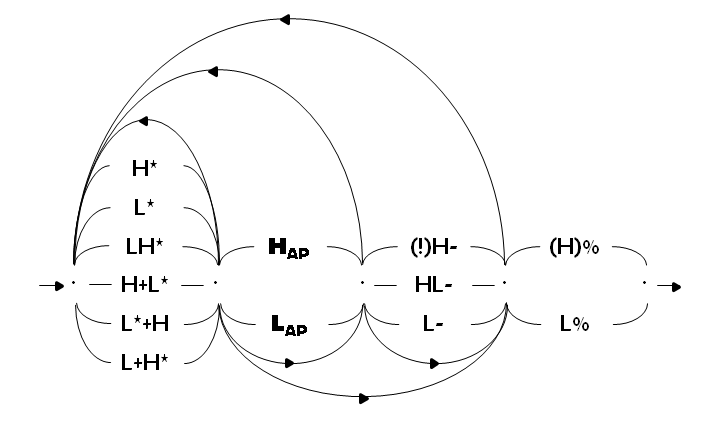
\includegraphics{images/212.png}}
\caption{AM intonational grammar for NI expanded with the Accentual Phrase level.}
\label{fig212}\end{figure}

Less effort is devoted to the phonological modelling of activating and restricting phrase final rises in German \cite{dombrowski2005acoustic}. The two phrase-final rises (concave and turn-holding, convex and turn-yielding) are treated as ``sub-patterns'' of the same ``contour type'', the early valley. The phonological inventory of the Kiel Intonation Model seems to be composed by a subset of the matrix created by two tonal movements (peaks and valleys) and three synchronization options (early, medial and late): as the authors put it, ``There are early, medial, and late peaks; and there are early and late (i.e., non-early) valleys''. It appears that the contrast between medial and late synchronizations options is neutralized when the tonal movement is a valley (see Figure~\ref{fig213} A). That is, the phonological inventory has an empty slot (i.e., medial valley) adjacent to the item (i.e., early valley) which displays the two sub-patterns (i.e., activating and restricting). Moreover, the activating and restricting sub-patterns of phrase-final early valleys are treated as ``coherent gestalt-like shapes'', as integral communicative gestures: the authors exclude the possibility of decomposing the rises in smaller unit, thus pointing to an inventory enrichment perspective. However, they do not take a clear position as for the restructuring of the inventory either. We could formulate two hypotheses here: in one case, we could distinguish between two sub-sub-types (concave and convex) in the sub-type (early) of the type (valley). This would entail the extrusion of another level (shape) in the already existing matrix (tonal movement x synchronization options), if only for one slot (see Figure~\ref{fig212} C). Alternatively, since (as we said earlier) medial valleys are not attested, the synchronization options could be broadened to account for shape differences as well, at least for non-early valleys (see Figure~\ref{fig212} B). These options of inventory enrichment are not explored in the original paper, but it appears that they would be less disruptive than a grammar enrichment anyway.

\begin{figure}
\centering
\resizebox{\linewidth}{!}{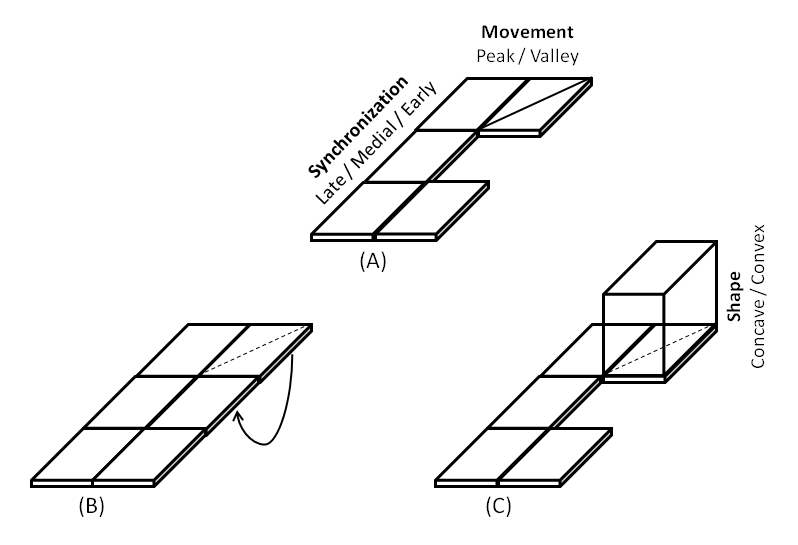
\includegraphics{images/213.png}}
\caption{KIM inventory (A) expanded by using the empty slot of medial valleys (B) or by extruding the matrix with the shape dimension (C).}
\label{fig213}\end{figure}

In the two studies cited above the issue of phonological modelling is either set and answered or not set at all: different prenuclear falls in Italian are due to a different Accentual Phrase tone, while phrase-final rises in German are two phonetic variants of the early valley. In the paper on prenuclear falls in German \citep{petrone2014intonation} the question is set but left unanswered. The authors suggest to interpret the differences in the shape of the fall as the consequence of the implementation of a tonal contrast, leaving open the possibilities of a trailing tone and an edge tone. The latter hypothesis clearly echoes the grammar enrichment proposed for prenuclear falls in Italian, and postulates the existence of a prosodic constituent smaller than the intermediate phrase for German as well. The former hypothesis, on the other hand, would introduce a distinction in the inventory between a prenuclear accent in statements (to be labelled as H*+L) and one in questions (H*+H or, with a ``crypto-phonetic'' labelling in the terms of \citealt{atterer2004phonetics}, H*+!H). It has to be noted that, when looking at Figure~\ref{fig211}, alignment differences in the prenuclear accent are evident, even if they only relate to two individual productions. In KIM terms, we would be dealing with a medial peak (statement) and a late peak (questions): again, shape differences could be fairly easily subsumed in the broader, holistic difference between two established phonological entities. This view would be supported by the fact that, while in AM accounts of at least some languages the inventory of prenuclear pitch accents is somehow reduced, in KIM different synchronization options are still available for prenuclear peaks \citep{niebuhr2006alignment}. However, in the examples of Figure~\ref{fig211} the alignment differences are somehow smaller than usually reported for the H* vs L*+H contrast (40 ms, against the 80 ms reported in \citealt{niebuhr2006alignment}). And the results from the second perception experiment in \citet{petrone2014intonation} show that stimuli with later prenuclear peaks do not yield more question responses. This finding seems actually to contradict the idea that the two sentence modalities might be characterized by two different prenuclear accents (medial peak, H* with convex fall for statements and late peak, L*+H with concave fall for questions). Conversely, manipulations of fall shape seem to yield different responses (more convex, more statement), but only when the peak has been manipulated to an early position (and the slope of the fall is not too steep). However, the hypothesis of true differences in the phonological inventory of German cannot be too hastily dismissed: as the authors point out, the interplay between shape, slope and alignment in the two postnuclear falls still needs a thorough investigation. The exaggeration of alignment differences might have proven disruptive indeed: after all, shape differences become a stronger cue to sentence modality when the peak is early and the slope is shallow - that is, when the perceptibility of shape differences is maximized. In sum, given also that the creation of the manipulated stimuli did not rely on the modelling of a conspicuous set of production data, it is difficult to decide whether an enrichment of the grammar or of the inventory would provide the best account of sentence modality perception.

\subsection{Segmental and suprasegmental phonology}\label{sec243}
But why would the issue of enriching inventories or grammars be so crucial in the refinement of phonological accounts of intonation? As we said in the opening pages of this chapter, it is a useful conceptual device to understand the relationships between the different phonological models of intonation. Moreover, it provides a link between models of intonation and of speech perception. But this issue is of central concern for another reason, namely the nature of the functions which can be expressed by intonational contrasts, as opposed to the functions played by phonemic contrasts. As \citeauthor{pierrehumbert1990meaning} put it, 
\begin{quote}
In the segmental domain, linguistic categories are expected to relate both to differences in sounds and articulations and to differences in semantic interpretation. For example, we say that [p] is different from [b] because they are pronounced differently, and because [pit] means something different than [bit] does. \cite[p. 282]{pierrehumbert1990meaning}
\end{quote}
In the suprasegmental domain, however, the establishment of phonological \textit{forms} (``linguistic categories'' in the quote) is less straightforward. First of all, intonational phonology is a very young field of study (especially if compared to segmental phonology) and no framework within it can be said to have reached the status of a stable system. For example, while the International Phonetic Alphabet has represented for years a valuable tool for research in segmental phonology, tonal transcription systems are still witnessing very partial consensus. But if it is true that intonational phonology is still very challenging because the first comprehensive modelling efforts only started some thirty years ago, the cause-effect relationship can also be flipped the other way round: intonation has eluded phonological modelling for a long time because of the many thorny issues it raises. A thorough examination of the reasons for the late inclusion of intonation in the core of linguistic studies is clearly beyond the scope of this chapter, so in the following we will only deal with the \textit{functional} issues (``semantic interpretation'' in the quote) which are immediately relevant to our discussion, but this reasoning could be very easily expanded to the difficulties raised by the \textit{substantial} aspects (``sounds and articulations'') of intonation.

\subsubsection{Solidity of functional contrasts}\label{sec2431}
In the quote, it is said that the establishment of phonological forms in the segmental domain (``[p] is different from [b]'')\footnote{Square brackets in the original text.} is guided by both substantial (``they are pronounced differently'') and functional (``[pit] means something different than [bit] does'') evidence. And, as the example in the quote shows, the functional evidence used in the establishment of forms in segmental (and tone) phonology is based on lexical semantic contrasts. These contrasts are characterized by a high degree of self-evidence, they are rooted in the epilinguistic knowledge of native speakers, and they do not require a theoretical systematization in order to be used as evidence for phonological contrasts. Of course, this is not to say that lexical semantic contrasts cannot be studied in their own right, but only that no semantic analysis is required when establishing a phonemic inventory. Pairs like the nouns \textit{bug} ([b\textipa{2}g], meaning ``insect'') and \textit{bun} ([b\textipa{2}n], meaning ``small cake'') allow for the individuation of the phonemes /g/ and /n/ irrespective of the fact that, as for their meanings, some semantic features are shared (e.g. [+organic]), some are not (e.g. [+animate]), and some could, depending on the context (e.g. [+edible]). 

In the suprasegmental domain, on the other hand, functional evidence used in the determination of phonological form does not share the immediacy of lexical (semantic) contrasts. For instance, non-linguists are not necessarily aware of the mechanisms underlying post-lexical contrasts such as differences in focus placement and scope, and there is no consensus on how to model them among linguists either. Also, from a cross-linguistic point of view, the role of intonation in conveying sentence modality contrasts such as the difference between statements and questions can range from essential (e.g. Italian) to marginal (e.g. mandarin Chinese, see \citealt{zeng2004tones}). Combined with the difficulties of analysis at the substantial level (e.g. microprosodic perturbations, measuring issues), the unavailability of rock-solid functional evidence makes the establishment of phonological forms in the suprasegmental domain a very complicate enterprise. Researchers in intonational phonology must treat functional post-lexical contrasts as nothing more than working hypotheses whereas, in segmental phonology, functional lexical contrasts can be used as solid guidelines for the exploration of differences in phonetic substance and for the definition of phonological forms. This might be one of the reasons underlying the (relatively) untroubled definition of the phoneme as the atomic unit at the segmental level. That is, the opposition between \textit{bug} and \textit{bun}, both at the functional and substantial level, is framed in the terms of the contrast between /g/ and /n/, and not in terms of the features of place and manner of articulation. Having clearly defined the atomic level, the constitution of the inventory results simplified. 

\subsubsection{Implicit compositionality of intonational meaning}\label{sec2432}
The \textit{f0} contour shape differences discussed in this chapter are a good example of how the definition of phonological form in intonation can be problematic, and of how the interplay between inventory and grammar is indeed crucial. If the definition of the inventory relies on the individuation of what we called the atomic level, what role should shape differences play? If tones are the primitives, then shape differences can be accounted for as different tonal specifications for a new structural position: the inventory stays the same, the grammar is enriched (see \citealt{petrone2008tonal}). If, on the other hand, tonal configurations are seen as gestalt-like atomic wholes (see \citealt{dombrowski2005acoustic}), the inventory has to be enriched by splitting a previously acknowledged slot (say KIM's early valley) into two novel forms, differentiated on the basis of the \textit{feature} of convexity/concavity.

The issue of the atomic level in intonational phonology is also relevant on the functional side. This can be exemplified by looking at the pragmatic contrast we explored in this chapter (see Section~\ref{sec212}), which we labelled as Partial Topic Statement (SPT) versus Narrow Focus Question (QNF). Is this functional contrast a viable starting point for the individuation of different phonological forms? The SPT vs QNF contrast is clearly multidimensional: sentence modality, focus placement, and topic contrastiveness all take different values in these two contexts. As we said in the preceding section, this is not an issue when dealing with functional contrasts on the segmental level, where the semantic features of the two items composing a minimal pair can safely be ignored, since the functional contrast is pre-theoretic and the atomic phonological level is clearly defined. But among the shifting sands of intonational phonology, where the interactions between inventory and grammar are still to be settled, the question has to be asked. To exemplify, no phonological account of the bug/bun contrast would suggest to relate the phonetic feature [+velar] with the semantic feature [+animate]. But in the discussion of phrase-final German rises, it appears that the phonetic feature [+convex] is related to the discourse feature [+activating]. And in the case of prenuclear Italian falls, the phonological option of a Low accentual phrase tone would relate the phonetic feature [+convex] with the sentence modality [+statement].

That is, given the provisional and theory-dependent nature of both post-lexical functions and atomic forms, it appears that theories of intonational meaning are prone to an implicit drift towards a compositional approach. A specific primitive might be seen as conveying different meaning on different dimension, depending on its role in the grammar: in the terms of  \citet{petrone2008tonal,grice2005strategy}, an L tone would cue continuation on the discourse dimension if it is a prenuclear accent, and it would cue statement on the modality dimension if it is an accentual phrase accent. Or, given a single primitive, different features might relate to different meaning dimensions: in \citet{dombrowski2005acoustic}, within the general case of early valleys, it is the feature of concavity or convexity that relates to restriction or activation of the interlocutor. These accounts are implicitly compositional in the weak sense that at least some of the meaning of the whole can be associated with options pertaining to one of its parts, and that these parts are at least partially meaningful on their own. That is, with respect to meaning, units in intonational phonology have been treated more like morphemes than phonemes \citep{gussenhoven1984grammar}. This is actually less surprising than expectable, since the arguments discussed in this section aimed to show that intonational phonology still hasn't located an atomic level comparable to the phoneme \textit{with respect to form and substance as well}. And that a closer examination of the relationships between inventory and grammar could represent a necessary step to this end.

\section{Conclusion}\label{sec25}
In this chapter we documented the production of melodic detail in read speech. Neapolitan Italian speakers produce nuclear rises with different shapes according to the pragmatic context of their utterances. Convex and concave rises are associated with narrow focus questions and partial topic statements, respectively. This phonetic information is a more reliable indicator of the QNF-SPT contrast than the traditional indices of tone scaling and alignment, but it is still unaccounted for in the autosegmental-metrical framework. That is, it is possible that phonological representations in the AM framework are too reductionists, and that they discard potentially useful prosodic detail. 

We explored some of the avenues for enriching these representations, keeping in mind that phonetic information can be included in a phonological description either through an increase in the inventory or through a stratification of the grammar. The exploration of these two hypotheses, illustrated also by other studies on meaningful contour shape differences, allowed us to recognize that the articulation between inventory and grammar in intonational phonology suffers from a constitutional instability, mainly due to the nature of the function expressed by intonational contrasts. The post-lexical meaning vehiculated by intonation does not share the immediacy and the pre-theoretic character of the lexical semantic contrasts used in segmental phonology. And this might have led to some difficulties in individuating an atomic bundle of relationship between substance and function parallel to the phoneme at the segmental level. In turn, this situation could have generated a more or less implicit drift towards a morpheme-like interpretation of intonational units, which informed a more or less overt compositional approach to intonational meaning. This is not, in itself, a problem for intonational phonology. However, the limits of an \textit{implicitly} compositional approach to meaning emerge when faced with the necessity of enriching phonological descriptions, because it is unclear whether the new features should be accounted for by an expansion of the inventory or a complexification of the grammar. In this sense, the accommodation of prosodic detail into an abstractionist model of intonation can prove challenging indeed. 

The elaboration of such a frame for the enrichment of phonological representations in an abstractionist model, and a fortiori the exploration of a potential exemplar-based approach of intonation, are not the aim of this chapter, nor of this book altogether. Our investigation bears mainly on asking \textit{whether} these enterprises are possible, useful or necessary. And as we said at the beginning of this chapter, in order to be considered as prosodic detail which must be included in a higher-order representation, phonetic variation must not only be regularly found in production, but also consistently used in perception. For this reason, in the next chapter we turn to an exploration of the perceptual role of differences in \textit{f0} contour shape.